\documentclass[]{book}

%These tell TeX which packages to use.
\usepackage{array,epsfig}
\usepackage{amsmath}
\usepackage{amsfonts}
\usepackage{amssymb}
\usepackage{amsxtra}
\usepackage{amsthm}
\usepackage{mathrsfs}
\usepackage{color}
\usepackage{graphicx}
\usepackage{float}

%Algorithm packages
\usepackage{algorithm}  
\usepackage{algpseudocode}  
\usepackage{amsmath}  
\renewcommand{\algorithmicrequire}{\textbf{Input:}}  % Use Input in the format of Algorithm  
\renewcommand{\algorithmicensure}{\textbf{Output:}} % Use Output in the format of Algorithm  
%Here I define some theorem styles and shortcut commands for symbols I use often
\theoremstyle{definition}
\newtheorem{defn}{Definition}
\newtheorem{thm}{Theorem}
\newtheorem{cor}{Corollary}
\newtheorem*{rmk}{Remark}
\newtheorem{lem}{Lemma}
\newtheorem*{joke}{Joke}
\newtheorem{ex}{Example}
\newtheorem*{soln}{Solution}
\newtheorem{prop}{Proposition}

\newcommand{\lra}{\longrightarrow}
\newcommand{\ra}{\rightarrow}
\newcommand{\surj}{\twoheadrightarrow}
\newcommand{\graph}{\mathrm{graph}}
\newcommand{\bb}[1]{\mathbb{#1}}
\newcommand{\Z}{\bb{Z}}
\newcommand{\Q}{\bb{Q}}
\newcommand{\R}{\bb{R}}
\newcommand{\C}{\bb{C}}
\newcommand{\N}{\bb{N}}
\newcommand{\M}{\mathbf{M}}
\newcommand{\m}{\mathbf{m}}
\newcommand{\MM}{\mathscr{M}}
\newcommand{\HH}{\mathscr{H}}
\newcommand{\Om}{\Omega}
\newcommand{\Ho}{\in\HH(\Om)}
\newcommand{\bd}{\partial}
\newcommand{\del}{\partial}
\newcommand{\bardel}{\overline\partial}
\newcommand{\textdf}[1]{\textbf{\textsf{#1}}\index{#1}}
\newcommand{\img}{\mathrm{img}}
\newcommand{\ip}[2]{\left\langle{#1},{#2}\right\rangle}
\newcommand{\inter}[1]{\mathrm{int}{#1}}
\newcommand{\exter}[1]{\mathrm{ext}{#1}}
\newcommand{\cl}[1]{\mathrm{cl}{#1}}
\newcommand{\ds}{\displaystyle}
\newcommand{\vol}{\mathrm{vol}}
\newcommand{\cnt}{\mathrm{ct}}
\newcommand{\osc}{\mathrm{osc}}
\newcommand{\LL}{\mathbf{L}}
\newcommand{\UU}{\mathbf{U}}
\newcommand{\support}{\mathrm{support}}
\newcommand{\AND}{\;\wedge\;}
\newcommand{\OR}{\;\vee\;}
\newcommand{\Oset}{\varnothing}
\newcommand{\st}{\ni}
\newcommand{\wh}{\widehat}

%Pagination stuff.
\setlength{\topmargin}{-.3 in}
\setlength{\oddsidemargin}{0in}
\setlength{\evensidemargin}{0in}
\setlength{\textheight}{9.in}
\setlength{\textwidth}{6.5in}
\pagestyle{empty}



\begin{document}


\begin{center}
{\Large COMP 540 \hspace{0.5cm} Homework 2}\\
\textbf{Peiguang Wang, Xinran Zhou}\\ %You should put your name here
Due: February 2, 2018 %You should write the date here.
\end{center}

\vspace{0.2 cm}

\subsection*{Part 1: Gradient and Hessian of $NLL(\theta)$ for logistic regression}
\begin{enumerate}
	\item
	Let $g(z)=\frac{1}{1-e^{-z}}$. Show that $\frac{\partial g(z)}{\partial z}=g(z)(1-g(z)).$
	\begin{proof}
		$$\frac{\partial g(z)}{\partial z} = -\frac{e^{-z}}{(1-e^{-z})} = \frac{1}{1+e^{-z}} (1 - \frac{1}{1+e^{-z}}) = g(z)(1-g(z))$$
	\end{proof}
	
	\item
	Using the previous result and the chain rule of calculus, derive the following expression for the gradient of the negative log likelihood function $NLL(\theta)$ for logistic
	regression.
	$$\frac{\partial }{\partial \theta} NNL(\theta)=\sum_{i = 1}^{m}(h_{\theta}(x^{(i)}) - y^{(i)})x^{(i)}$$
	
	\begin{proof}
		Let $h_{\theta}$ denote $h_{\theta}(x^{(i)})$. Then the $NLL(\theta)$ is:
		$$NLL(\theta) = - \frac{1}{m} \sum_{i = 1}^{m} y^{(i)} log(h_{\theta}) + (1-y^{(i)})log(1-h_{\theta})$$
		Then
		$$\frac{\partial }{\partial (\theta x) } NNL= - \sum_{i = 1}^{m} y^{(i)} \frac{h_{\theta}(1 - h_{\theta})}{h_{\theta}} + (-1)(1 - y^{(i)} \frac{h_{\theta}(1 - h_{\theta})}{1 - h_{\theta}})$$
		Simplify the equation above
		$$\frac{\partial }{\partial (\theta x) } NNL= - \sum_{i = 1}^{m} y^{(i)} (1 - h_{\theta}) + (y^{(i)} - 1) h_{\theta} = -\sum_{i = 1}^{m} y^{(i)} - h_{\theta}$$
		Derive $\frac{\partial }{\partial (\theta) } NNL $ from $\frac{\partial }{\partial (\theta x) } NNL $:
		$$\frac{\partial NNL }{\partial \theta } = \frac{\partial NLL }{\partial (\theta x) } \frac{\partial (\theta x)}{\partial \theta } = \sum_{i = 1}^{m}(h_{\theta}(x^{(i)}) - y^{(i)})x^{(i)}$$
		
	\end{proof}
	
	\item 
	The Hessian or second derivative of the $NLL(\theta)$ can be written as $H=X^{T}SX$ where
	$$S=diag(h_{\theta}(x^{(1)})(1-h_{\theta}(x^{(1)})),...,h_{\theta}(x^{(m)})(1-h_{\theta}(x^{(m)})))$$
	
	Show that $H$ is positive definite. You may assume that $0 < h_{\theta}(x^{(i)}) < 1$, so the elements of $S$ are strictly positive and that $X$ is full rank.
	
	\begin{proof}
		For any given vector $u$, compute $u^THu$:
		$$u^THu = u^TX^TSXu $$
		Let vector $v = (v_1, v_2,...v_m)$ denote $X\dot u$. since $X$ is full rank, then $v$ is not a zero vector.
		$$u^THu = v^TSv = \sum_{i=1}{m} v_i^2S_{ii}$$
		Since the elements of $S$ are strictly positive, then $u^THu > 0$. So $H$ is positive definite.
	\end{proof}
	
\end{enumerate}

\subsection*{Part 2: Properties of L2 regularized logistic regression }
\begin{enumerate}
	\item (True or False) $J(\theta)$ has multiple locally optimal solutions.
	\begin{soln}
		This statement is \textbf{False}. Since $J(\theta)$ is a convex function, it only have one global optimal point.
	\end{soln}
	
	\item (True or False) Let $\theta^{\star} = argmin_{\theta}J(\theta)$ be a global optimum. $\theta^{\star}$ is sparse (has many zero entries).
	\begin{soln}
		This statement is \textbf{False}. Since in this regression problem, we use L2 regularization, it won't make $\theta^{\star}$ become sparse. L2 norm will make $\theta$ have small values. If L1 norm is used, then $\theta^{\star}$ will become sparse.
	\end{soln}
	
	\item (True or False) If the training data is linearly separable, then some coefficients $\theta_j$ might become infinite if $\lambda = 0$.
	\begin{soln}
		This statement is \textbf{True}. When the
		 maximum likelihood solution occurs, sigmoid function is equal to 0.5, which means that $ \theta_j^T x = 0 $, the magnitude of $\theta_j$ goes to infinity.
	\end{soln}
	\item (True of False) The first term of $J(\theta)$ always increases as we increase $\lambda$.
	\begin{soln}
		This statement is \textbf{True}. When adding $\lambda$, the cross-entropy loss
		$$J = - \frac{1}{m} \sum_{i = 1}^{m} y^{(i)} log(h_{\theta}(x^{(i)})) + (1-y^{(i)})log(1-h_{\theta}(x^{(i)}))$$
		will become larger to prevent overfitting.
	\end{soln}
	
\end{enumerate}

\subsection*{Part 3: Implementing a k-nearest-neighbor classifier}
\begin{enumerate}
	\item Distance matrix computation with two loops.
	\begin{soln}
		To solve the problem using two loops, we just compute the distance between the $i^{th}$ test set example and the $j^{th}$ training example, and put that value into $dists(i,j)$.\\
		1. In the image, each row corresponds to the distances between a specific test example to all the training examples. If a point is bright, it means that the distance is larger than others. So the distinctly bright rows in the image means that: for those test examples, the distance between those and all the training examples are large. Those test samples are more different than others when compared to training examples. Maybe these test examples aren't from any of the classes. Or maybe the test examples are hard to classify.\\
		2. Similarly, the columns is caused by the fact that, the training examples are different from almost all the test examples.
	\end{soln}
	\item Computer majority label.
	\begin{soln}
		Result for $k = 1$: Got 137 $/$ 500 correct $=>$ accuracy: 0.274000.\\
		Result for $k = 5$: Got 139 $/$ 500 correct $=>$ accuracy: 0.278000.\\
		We can see that there is a slightly better performance for $k = 5$than with $k = 1$.
		\end{soln}
	\item Distance matrix computation with one loop.
	\begin{soln}
		Compared to two loops, we compute one entire training data set each time instead of a single example. The result shows that our result is the same as that using two loops. Difference was: 0.000000. Good! The distance matrices are the same 
	\end{soln}
	\item Distance matrix computation with no loop.
	\begin{soln}
		The idea comes for the simple equation $(a-b)^2 = a^2 + b^2 - 2 ab$. For two matrix we can use the similar method, so we need to do one matrix multiplication, and then do two broadcast sums, which are the square of the two matrix.\\
		The result is same compared to the former methods. We can compare how fast the implementations are. The result is that:\\
		Two loop version took 884.739000 seconds\\
		One loop version took 104.597000 seconds\\
		No loop version took 12.769000 seconds
	\end{soln}
	\item Choosing k by cross validation.
	\begin{figure}[h]
			\centering
			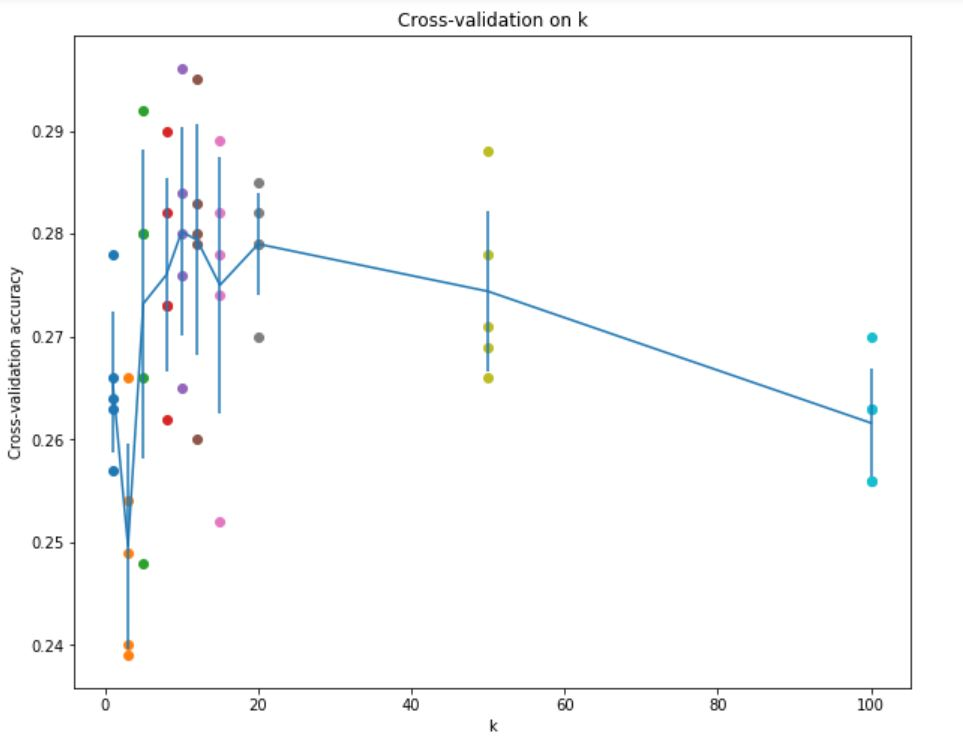
\includegraphics[width=11cm]{knn.jpg}
			\caption{Choosing k by crossvalidation on the CIFAR-10 dataset}
			\label{fig:1}
	\end{figure}
	\begin{soln}
		by applying cross-validation, we can get a set of accuracies for all folds. And by changing the value of k, we can also have different accuracies which corresponding to different k.\\
		According to the plot, we choose $k=8$ as our best value for k and then use this value to retrain the model. We get:\\
		Got 141 $/$ 500 correct $=>$ accuracy: 0.282000. \\It shows that when $k = 8 $ the result is better than other values we have used. 
	\end{soln}
\end{enumerate}

\subsection*{Part 4: Implementing logistic regression}
\subsection*{Problem 3A3: Prediction using a logistic regression model}
The decision boundaries drawn by our logistic regression program and sklearn are shown in figure \ref{fig:boundary}. Left is the linear boundary drawn by our program. Right is the linear boundary drawn by sklearn package. Results of these two methods are similar.
\begin{figure}[H]
	\centering
	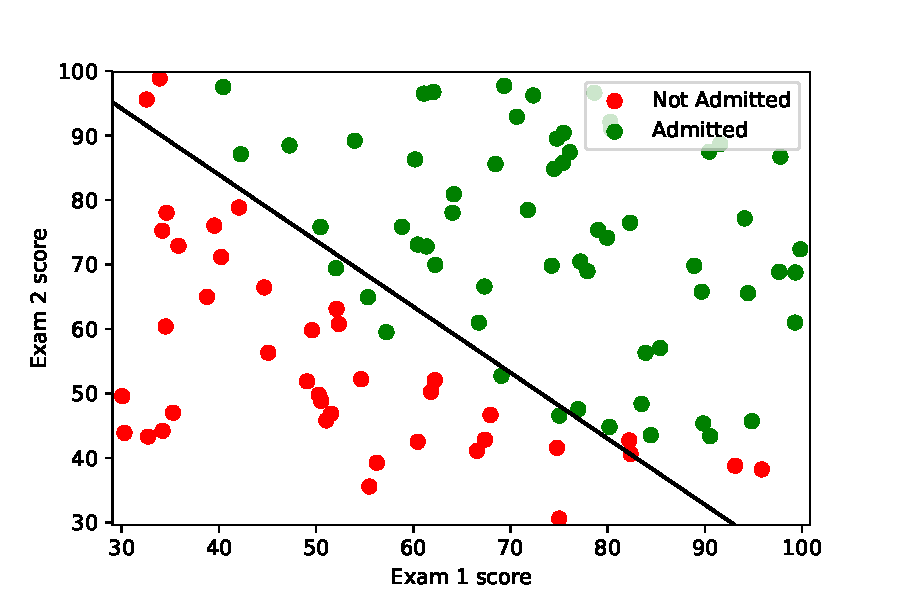
\includegraphics[width=7cm]{imgs//boundary_1.pdf}
	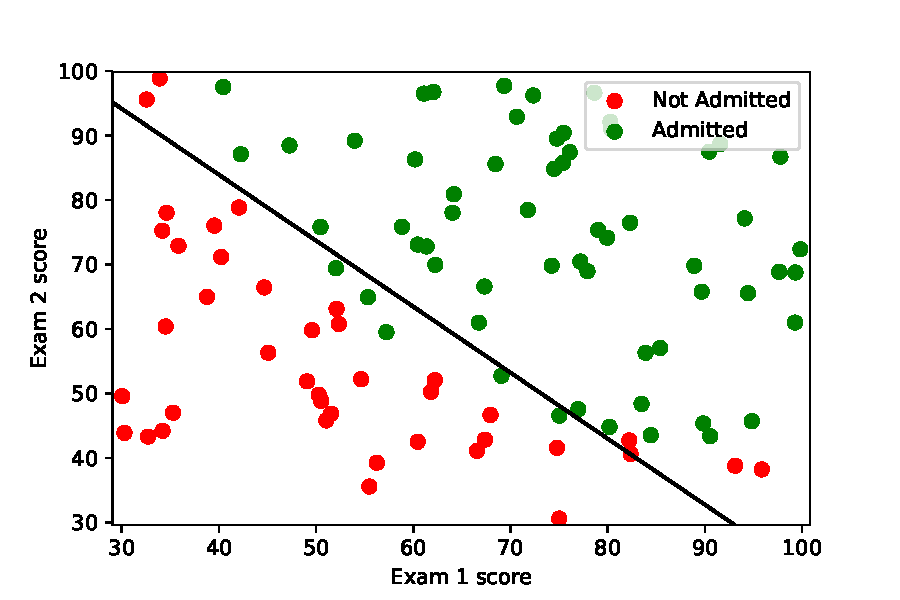
\includegraphics[width=7cm]{imgs//boundary_sk.pdf}
	\caption{Linear boundaries drawn by our program and by sklearn. Left is the linear boundary drawn by our program. Right is the linear boundary drawn by sklearn package. Results of these two methods are similar.}
	\label{fig:boundary}
\end{figure}

\subsection*{Problem 3B3: Varying $\lambda$}
Adjusting different $\lambda$, you will see different models. When $\lambda$ is very large, the model becomes underfitting. When $\lambda$ is very small(close to zero), the model becomes overfitting. Figure \ref{fig:Overfit_Underfit} shows results under different $\lambda$. Left shows the underfitting model ($\lambda = 100$). Right shows the overfitting model ($\lambda$ = 1e-6).
\begin{figure}[H]
	\centering
	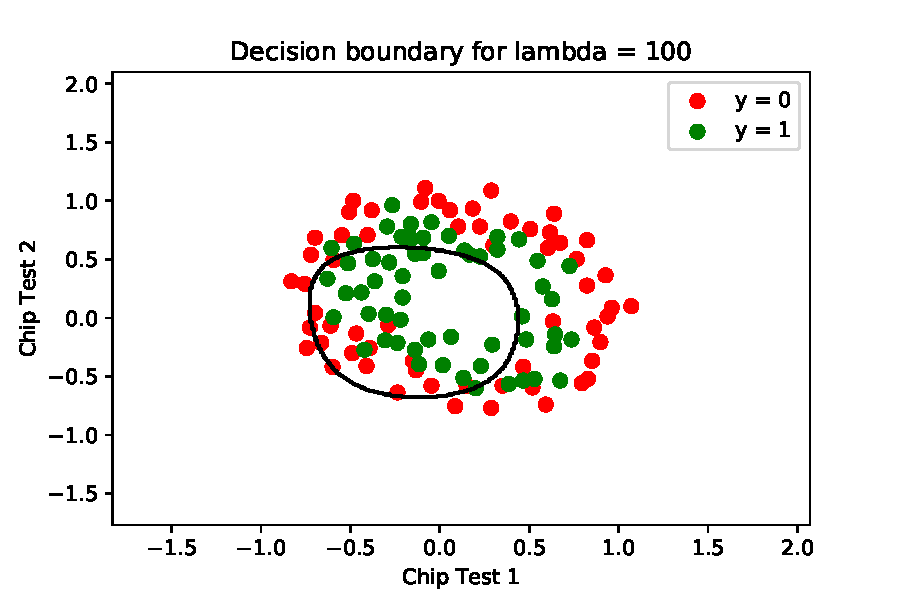
\includegraphics[width=7cm]{imgs//underfitting.pdf}
	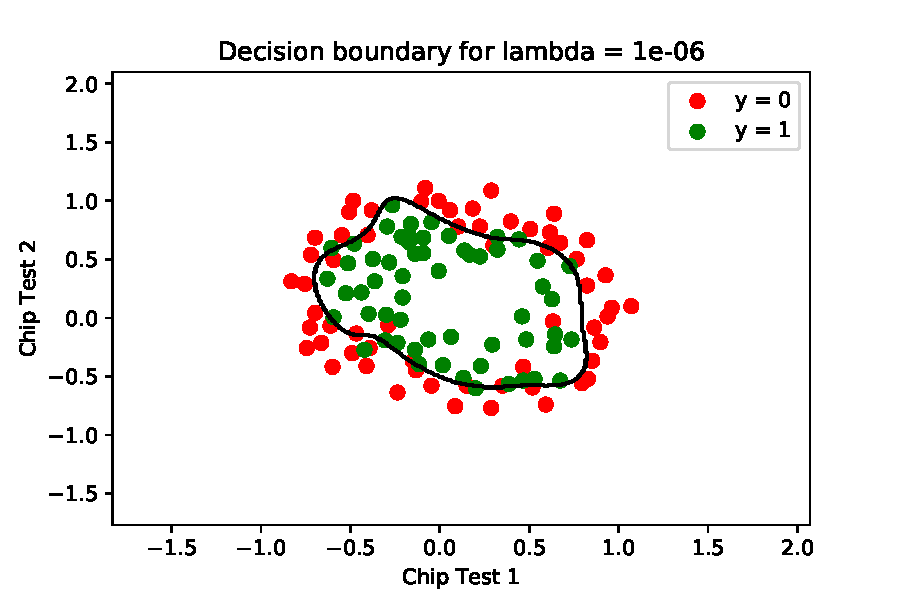
\includegraphics[width=7cm]{imgs//overfitting.pdf}
	\caption{Linear boundaries drawn by our program and by sklearn. Left shows the underfitting model ($\lambda = 100$). Right shows the overfitting model ($\lambda$ = 1e-6).}
	\label{fig:Overfit_Underfit}
\end{figure}

\subsection*{Problem 3B4: Exploring L1 and L2 penalized logistic regression}
Compare L1 and L2 penalized logistic regression with different $\lambda$. The results are shown in table \ref{tab:L1_L2}
\begin{table}[H]
	\centering
	%\ref{tab:L1_L2}
	\begin{tabular}{ccccc}
		\hline 
		$\lambda$ & L1 Loss & L2 Loss & L1 non-zero $\theta$ & L2 non-zero $\theta$ \\ 
		\hline 
		0.01 & 0.2912 & 0.3167 & 19 & 28 \\ 
		
		0.1 & 0.3364 & 0.3538 & 14 & 28 \\ 
		
		0.3 & 0.3573 & 0.3946 & 8 & 28 \\ 
		
		1 & 0.4382 & 0.4684 & 7 & 28 \\ 
		
		3 &  0.6137 & 0.5496 & 3 & 28 \\ 
		
		10 & 0.6931 & 0.6216 & 0 & 28 \\ 
		\hline 
	\end{tabular} 
	\caption{Loss and number of non-zero parameters when varying $\lambda$}
	\label{tab:L1_L2}
\end{table}
As we can see from the table. We can draw some conclusions:
\begin{itemize}
	\item When $\lambda$ increases, the loss of both models increases.
	\item L1 penalty term makes the model sparse. The larger the $\lambda$ is, the less non-zero parameters in the trained model. However, L2 penalty term doesn't have this property.
	\item Loss in L1 model increases more quickly than L2 model. 
\end{itemize}

\subsection*{Fitting regularized logistic regression models (L2 and L1)}
\begin{enumerate}
	\item  Do this for every $\lambda$ in the swept range and return the lambda that yields the highest accuracy.
	\begin{soln}
		Please see the results in table \ref{tab:results}
		\begin{table}[H]
			\centering
			%\ref{tab:L1_L2}
			\begin{tabular}{cccc}
				\hline 
				Regularization & Feature & Best $\lambda$ & Accuracy \\ 
				\hline
				L2 & standard feature & 0.1 &0.9297   \\ 
				
				L2 & log-transformed & 0.6 &0.9434   \\ 
				
				L2 & binarized feature& 1.6 &0.9284   \\ 
				
				L1 & standard feature & 4.6 &0.9219   \\ 
				
				L1 & log-transformed & 1.6 &0.9440   \\ 
				
				L1 & binarized feature& 3.6 & 0.9258  \\
				\hline 
			\end{tabular} 
			\caption{Loss and number of non-zero parameters when varying $\lambda$}
			\label{tab:results}
		\end{table}
	\end{soln}
	
	\item Comment on the model sparsities with L1 and L2 regularization. Which class of models will you recommend for this data set and why?
	\begin{soln}
		Please see model sparsity table in table \ref{tab:sparsity}. The results under L2 regularization are always dense. When using L1 regularization, results in log-transformed features are more sparse than standard features. And results with binarized features are more sparse than log-transformed features.
		\begin{table}[H]
			\centering
			%\ref{tab:L1_L2}
			\begin{tabular}{cccc}
				\hline 
				& \# of zeros (std) & \# of zeros (log) & \# of zeros(bin) \\ 
				\hline 
				L1 regularization & 4 & 15 & 20 \\ 
				
				L2 regularization & 0 & 0 & 0 \\ 
				\hline 
			\end{tabular} 
			\caption{Loss and number of non-zero parameters when varying $\lambda$}
			\label{tab:sparsity}
		\end{table}
		
		\noindent
		I will recommend the model using log transformed feature with L1 regularization($\lambda = 1.6$). Because the accuracy is the highest. And also has many zero parameters and therefore the model is less complex. 
	\end{soln}
	
\end{enumerate}



\end{document}


